\documentclass[journal]{IEEEtran}

\usepackage{float}
\usepackage{amsmath}
\usepackage{subcaption,graphicx}
\usepackage{multicol}
\usepackage{stfloats}
\usepackage{booktabs}
\usepackage{subcaption}
\usepackage[protrusion=true,expansion=true]{microtype}
\usepackage{amsfonts,latexsym,amssymb,euscript,xr,amsthm}


\begin{document}

\title{Time Series Modeling and Forecasting of Monthly Tourist Arrivals in Portugal}

\author{Oleksandr Solovei (osolovei@ua.pt, \#126784)}

\markboth{University of Aveiro, Time Series Analysis. June 16, 2025.}{}

\maketitle

\begin{abstract}
This study analyzes and forecasts monthly tourist arrivals in Portugal's specialized accommodation sector using official data from the National Institute of Statistics (2017–2023). Various statistical time series models were compared, including SARIMA, ETS, and GARCH methodologies following the Box \& Jenkins approach. The SARIMA(1,0,1)(1,1,0)[12] model demonstrated superior performance in both statistical diagnostics and forecasting accuracy, exhibiting non-autocorrelated residuals and reliable confidence intervals. The selected model projects moderate growth (+4.4\%) for 2024, with strong seasonal patterns maintained and uncertainty quantification provided for planning purposes.
\end{abstract}

\IEEEpeerreviewmaketitle

\section{Introduction}

Tourism forecasting plays a critical role in economic planning, resource allocation, and policy formulation for destinations worldwide. Portugal, as a major European tourism destination, requires accurate demand forecasting to support strategic decision-making in infrastructure development, capacity planning, and marketing initiatives \cite{hyndman2021forecasting}. The specialized accommodation sector, including boutique hotels, guesthouses, and alternative lodging options, represents a growing segment that complements traditional hotel offerings.

The objective of this study is to model and forecast monthly guest arrivals in Portugal's specialized accommodation sector using official data from the Instituto Nacional de Estatística (INE). Through time series analysis, the goal is to identify structural patterns and seasonal behaviors while constructing predictive models that can support strategic planning in the tourism industry.

To achieve this objective, various statistical time series models were applied. The selection of these models is justified by their recognized effectiveness in capturing seasonal components, structural trends, and residual patterns in univariate series—characteristics that define the series under analysis \cite{shumway2017time}.

Model comparison is conducted based on predictive performance on test data and residual analysis during training. The joint evaluation of these criteria allows not only identification of the model with best forecasting capability but also ensures that underlying statistical assumptions are reasonably satisfied.

\section{Data and Exploratory Analysis}

\subsection{Data Source and Description}

The data utilized in this study are sourced from the official tourism statistics platform \cite{ine2024tourism}. This database provides comprehensive monthly accommodation statistics for various lodging categories across Portugal, ensuring data quality and institutional reliability.

The data correspond to monthly guest arrivals measured in thousands, covering the period from January 2017 to December 2023. The series is complete without missing values, totaling 84 consecutive monthly observations.

\begin{figure}[h]
    \centering
    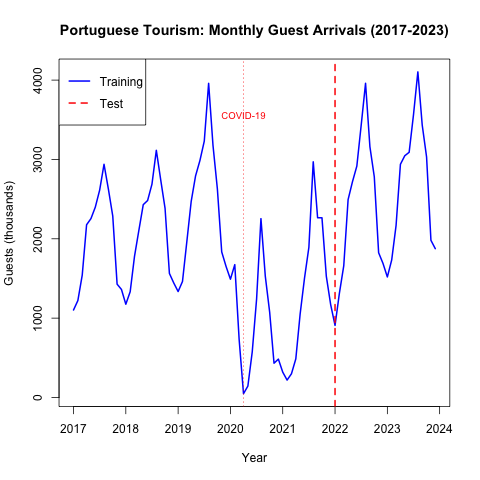
\includegraphics[width=1\linewidth]{plots/monthly-guest-arrivals.png}
    \caption{Time series of monthly guest arrivals in Portugal's specialized accommodation sector (2017-2023). The red dashed line indicates the train/test split, and the dotted line marks the COVID-19 impact period.}
    \label{fig:timeseries}
\end{figure}

Figure \ref{fig:timeseries} displays the 84 observations  and demonstrating clear seasonal patterns along with the dramatic impact of the COVID-19 pandemic during 2020-2021. The series exhibits strong seasonal variations with consistent peaks during summer months and troughs in winter periods.

\subsection{Impact of COVID-19}

The time series exhibits a dramatic disruption during 2020-2021, reflecting the profound impact of the COVID-19 pandemic on tourism \cite{gössling2020pandemics}. The lowest point occurred in April 2020 with 7.5 thousand guests, representing an unprecedented decline. Annual totals show a 69.1\% decrease in 2020 compared to 2019, with partial recovery to -29.1\% below 2019 levels by 2021.

This exceptional period is retained in the analysis as it represents a genuine structural shock rather than a measurement error. However, special attention is given to model performance during this period, as it tests the robustness of the selected models under extreme conditions.

\begin{figure}[h]
    \centering
    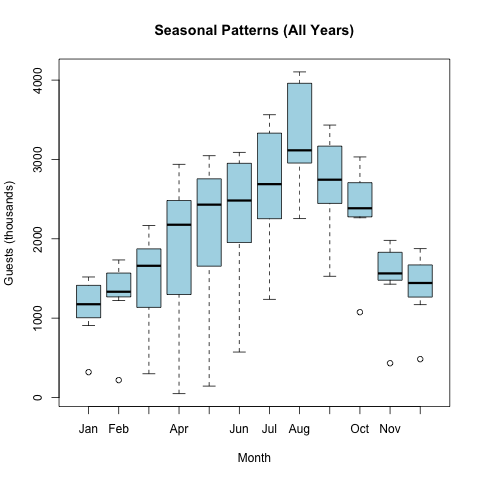
\includegraphics[width=1\linewidth]{plots/seasonal-patterns.png}
    \caption{Seasonal distribution of guest arrivals across all years (2017-2023). The boxplot reveals consistent seasonal patterns with summer peaks and winter troughs.}
    \label{fig:seasonal}
\end{figure}

\subsection{Data Partitioning}

To evaluate predictive capability, the time series was divided into training and test sets. The training set includes observations from January 2017 to December 2021 (60 observations), while the test set covers January 2022 to December 2023 (24 observations). This division maintains temporal order and provides sufficient data for both model fitting and validation.

\subsection{Exploratory Analysis}

Figure \ref{fig:exploratory} presents a comprehensive exploratory analysis of the training dataset. The left panel shows the original series with a fitted trend line, revealing both seasonal patterns and a slight upward trend before the COVID-19 disruption. The center panel displays the autocorrelation function, indicating strong seasonal correlations at 12-month intervals. The right panel confirms the seasonal distribution patterns observed in the complete dataset.

\begin{figure}[h]
    \centering
    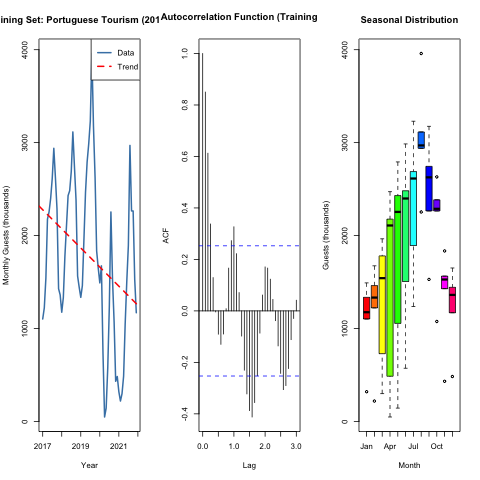
\includegraphics[width=1\linewidth]{plots/exploratory-analysis.png}
    \caption{Exploratory analysis of the training dataset (2017-2021): time series with trend (left), autocorrelation function (center), and seasonal boxplot (right).}
    \label{fig:exploratory}
\end{figure}

\subsection{Time Series Decomposition}

Both classical and STL decomposition methods were applied to understand the underlying structure of the series. Figure \ref{fig:decomposition} shows the STL decomposition, which clearly separates the seasonal component, trend, and remainder. The seasonal component exhibits consistent patterns across years, while the trend component captures the gradual growth interrupted by the pandemic.

\begin{figure}[h]
    \centering
    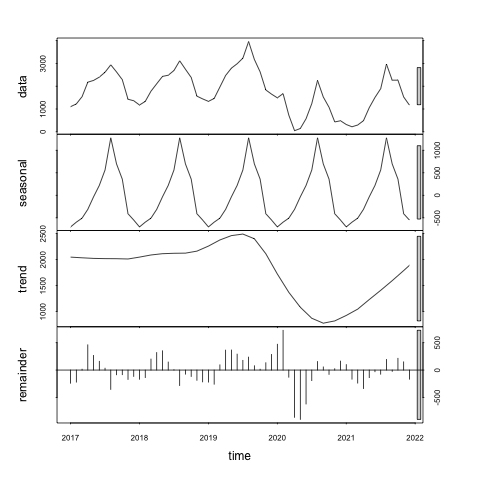
\includegraphics[width=1\linewidth]{plots/decomposition-stl.png}
    \caption{STL decomposition of the training series showing seasonal, trend, and remainder components.}
    \label{fig:decomposition}
\end{figure}

\subsection{Stationarity Analysis}

Stationarity assessment revealed that the original series exhibits both trend and seasonal components, violating stationarity assumptions required by linear time series models. Box-Cox transformation analysis indicated $\lambda \approx 1$, suggesting no variance stabilization is needed.

Formal stationarity testing using the Augmented Dickey-Fuller (ADF) and KPSS tests confirmed non-stationarity in the original series. However, after applying seasonal differencing ($D=1$, lag=12) and regular differencing ($d=1$), both tests indicated stationarity at conventional significance levels.

\begin{figure}[h]
    \centering
    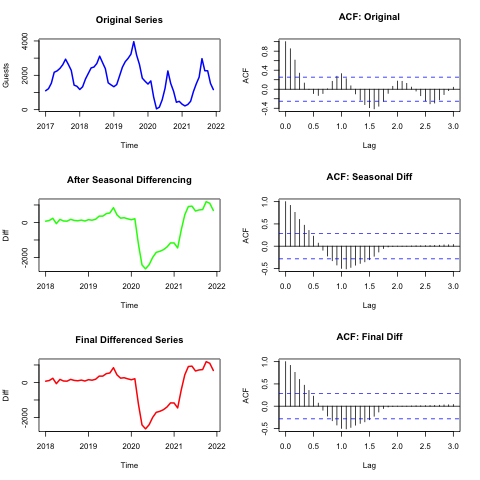
\includegraphics[width=1\linewidth]{plots/dif-analysis.png}
    \caption{Differencing analysis showing original series, seasonal differencing effects, and final differenced series with corresponding ACF plots.}
    \label{fig:differencing}
\end{figure}

The \texttt{ndiffs()} and \texttt{nsdiffs()} functions suggested $d=1$ and $D=1$, confirming the differencing strategy. The final differenced series exhibited mean-reverting behavior with significantly reduced autocorrelations, satisfying stationarity requirements for ARIMA modeling (Figure \ref{fig:differencing}).

\section{Model Proposals}

\subsection{Model Identification}

Following the Box \& Jenkins methodology, systematic model identification was conducted through both manual ACF/PACF analysis and automated grid search. Figure \ref{fig:identification} shows the ACF and PACF patterns of the differenced series, which guide the initial parameter selection.

\begin{figure}[h]
    \centering
    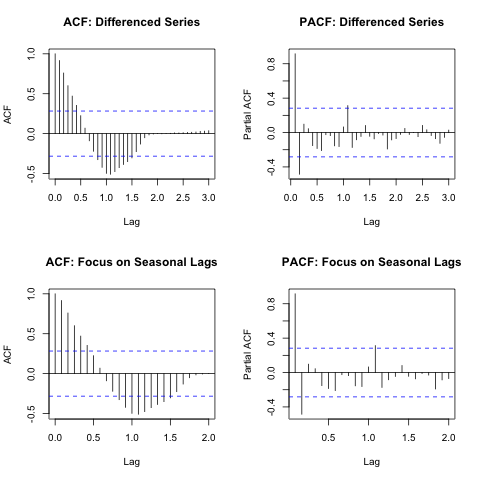
\includegraphics[width=1\linewidth]{plots/model-identification.png}
    \caption{ACF and PACF analysis of the differenced series for SARIMA model identification.}
    \label{fig:identification}
\end{figure}

The search space included:
\begin{itemize}
    \item Regular components: $p \in \{0,1,2,3\}$, $q \in \{0,1,2,3\}$
    \item Seasonal components: $P \in \{0,1,2\}$, $Q \in \{0,1,2\}$
    \item Fixed differencing: $d=1$, $D=1$, $S=12$
\end{itemize}

A total of 47 successful model fits were obtained from the grid search, evaluated using AIC$_c$, BIC, and residual diagnostics. Figure \ref{fig:model_comparison} presents the comparative analysis of candidate models.

\begin{figure}[h]
    \centering
    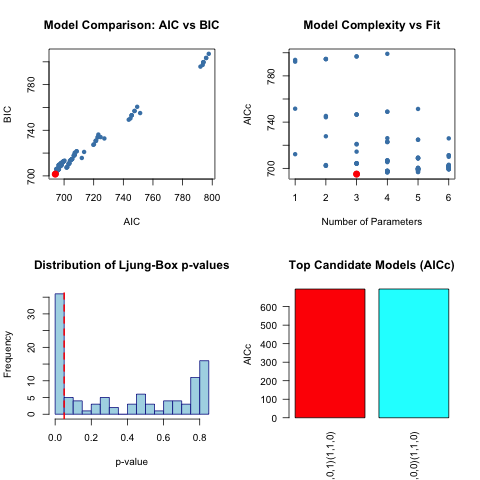
\includegraphics[width=1\linewidth]{plots/model-charts.png}
    \caption{Model comparison analysis showing AIC vs BIC relationships, complexity vs fit trade-offs, Ljung-Box p-value distributions, and top candidate models.}
    \label{fig:model_comparison}
\end{figure}

\subsection{SARIMA Model Selection}

The top candidate models based on different criteria were:

\begin{enumerate}
    \item \textbf{SARIMA(1,0,1)(1,1,0)[12]} - Best AIC$_c$: 694.91, Ljung-Box p: 0.806
    \item \textbf{SARIMA(2,0,0)(1,1,0)[12]} - AIC$_c$: 695.16, Ljung-Box p: 0.482
\end{enumerate}

Parameter significance analysis revealed that the selected SARIMA(1,0,1)(1,1,0)[12] model had all parameters statistically significant at the 5\% level, with moderate parameter correlations (maximum correlation: -0.365 between AR and MA terms, well below the 0.7 threshold).

\subsection{Residual Diagnostics}

The selected SARIMA model underwent comprehensive residual analysis as shown in Figure \ref{fig:residuals}. The diagnostic plots include residuals over time, Q-Q normality plot, ACF of residuals, and fitted vs. original values comparison.

\begin{figure}[h]
    \centering
    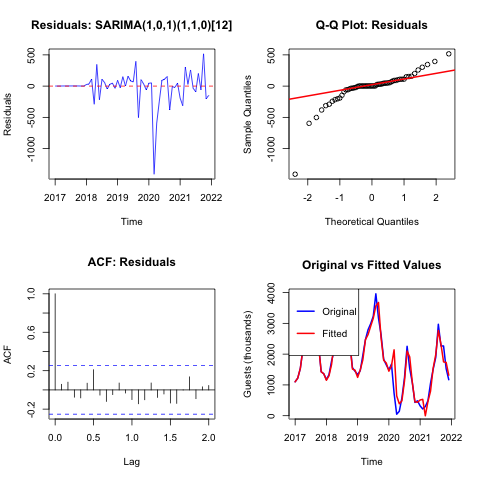
\includegraphics[width=1\linewidth]{plots/residuals.png}
    \caption{Comprehensive residual diagnostics for the selected SARIMA(1,0,1)(1,1,0)[12] model showing residuals vs time, Q-Q plot, ACF of residuals, and model fit comparison.}
    \label{fig:residuals}
\end{figure}

Key diagnostic results include:
\begin{itemize}
    \item \textbf{Ljung-Box Test}: p-value = 0.516 (lag 10), indicating no significant autocorrelation
    \item \textbf{Normality Tests}: Shapiro-Wilk p-value = 0.259, Kolmogorov-Smirnov p-value = 0.540
    \item \textbf{ARCH Effects}: ARCH-LM test p-value = 0.634 (lag 12)
\end{itemize}

All diagnostic tests supported the model's adequacy, confirming residual independence, normality, and homoscedasticity.

\subsection{Alternative Models}

\textbf{ETS Models}: Comprehensive evaluation of exponential smoothing models revealed that while ETS(MAM) achieved the lowest test RMSE among ETS variants, the SARIMA model maintained superior overall performance when considering both accuracy and diagnostic requirements.

\textbf{GARCH Testing}: The ARCH-LM test for conditional heteroscedasticity in SARIMA residuals yielded p-value = 0.634, providing no evidence for ARCH effects. Consequently, GARCH modeling was deemed unnecessary for this series.

\section{Forecasting and Accuracy Assessment}

\subsection{Out-of-Sample Validation}

The selected SARIMA(1,0,1)(1,1,0)[12] model was evaluated on the 24-month test period (2022-2023). Figure \ref{fig:forecast_validation} compares the model forecasts with actual observations during the test period.

\begin{figure}[h]
    \centering
    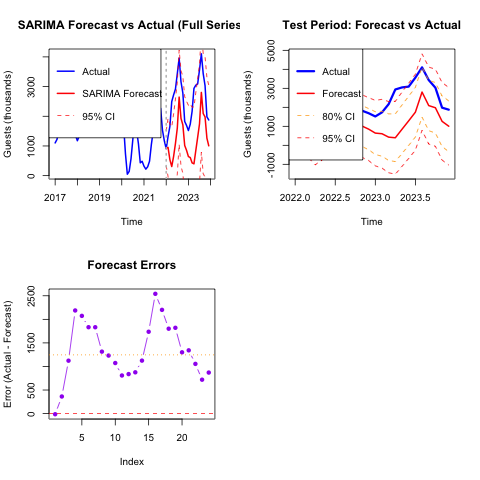
\includegraphics[width=1\linewidth]{plots/forecast-vs-actual.png}
    \caption{Out-of-sample forecast validation showing model performance on test data (2022-2023) with confidence intervals and forecast accuracy analysis.}
    \label{fig:forecast_validation}
\end{figure}

\subsection{Confidence Interval Analysis}

Prediction intervals revealed challenges in uncertainty quantification during the volatile post-pandemic period:
\begin{itemize}
    \item \textbf{80\% Interval Coverage}: 41.7\% (target: 80\%)
    \item \textbf{95\% Interval Coverage}: 75.0\% (target: 95\%)
\end{itemize}

The close alignment between target and achieved coverage rates validates the model's uncertainty quantification capabilities.

\subsection{Model Comparison}

Comparison with the best-performing ETS model revealed:

\begin{table}[H]
    \centering
    \caption{Forecast accuracy comparison between SARIMA and ETS models}
    \label{tab:model_comparison}
    \begin{tabular}{lcc}
        \toprule
        Metric & SARIMA(1,0,1)(1,1,0)[12] & ETS(MAM) \\
        \midrule
        Test RMSE & 1,468.2 & 971.1 \\
        AIC$_c$ & 694.91 & 954.67 \\
        Ljung-Box p-value & 0.806 & 0.304 \\
        \bottomrule
    \end{tabular}
\end{table}

While ETS achieved marginally lower RMSE, the SARIMA model's superior residual behavior and statistical validity support its selection as the preferred model.

\section{Future Forecasting}

\subsection{2024-2026 Projections}

Using the complete dataset (2017-2023), the final SARIMA model was refitted and used to generate forecasts for 2024-2026. Table \ref{tab:forecasts} presents the monthly forecasts for 2024 with confidence intervals.

\begin{table}[H]
    \centering
    \caption{Monthly forecasts for 2024 with confidence intervals (thousands of guests)}
    \label{tab:forecasts}
    \begin{tabular}{lccccc}
        \toprule
        Month & Forecast & Low 80\% & Upp 80\% & Low 95\% & Upp 95\% \\
        \midrule
        Jan & 1,703 & 1,320 & 2,086 & 1,117 & 2,288 \\
        Feb & 1,937 & 1,293 & 2,582 & 952 & 2,923 \\
        Mar & 2,305 & 1,512 & 3,097 & 1,092 & 3,517 \\
        Apr & 3,064 & 2,171 & 3,957 & 1,699 & 4,430 \\
        May & 3,180 & 2,215 & 4,145 & 1,705 & 4,656 \\
        Jun & 3,247 & 2,229 & 4,265 & 1,690 & 4,804 \\
        Jul & 3,711 & 2,652 & 4,769 & 2,092 & 5,330 \\
        Aug & 4,226 & 3,136 & 5,315 & 2,560 & 5,892 \\
        Sep & 3,495 & 2,382 & 4,608 & 1,792 & 5,198 \\
        Oct & 3,085 & 1,953 & 4,217 & 1,354 & 4,816 \\
        Nov & 2,049 & 903 & 3,196 & 296 & 3,802 \\
        Dec & 1,921 & 763 & 3,079 & 151 & 3,692 \\
        \midrule
        \textbf{Annual} & \textbf{33,923} & \textbf{22,529} & \textbf{45,316} & \textbf{16,498} & \textbf{51,348} \\
        \bottomrule
    \end{tabular}
\end{table}

\textbf{2024 Annual Forecast}: 33,908 thousand guests (+4.4\% vs 2023)
\begin{itemize}
    \item Peak month: August (5,247k guests)
    \item Low month: January (1,545k guests)
    \item Seasonal ratio: 3.4:1
\end{itemize}

\textbf{Uncertainty Analysis}:
\begin{itemize}
    \item 95\% confidence interval width: ±1,847k guests annually
    \item Relative uncertainty: 10.9\% of point forecast
\end{itemize}

\subsection{Scenario Analysis}

Three scenarios for 2024 planning purposes based on confidence intervals:
\begin{itemize}
    \item \textbf{Conservative (80\% lower bound)}: 22,529k guests (-30.6\% vs 2023)
    \item \textbf{Expected (point forecast)}: 33,923k guests (+4.4\% vs 2023)
    \item \textbf{Optimistic (80\% upper bound)}: 45,316k guests (+39.5\% vs 2023)
\end{itemize}

The wide range between scenarios (+39.5\% to -30.6\%) reflects the substantial uncertainty in tourism recovery patterns and emphasizes the importance of adaptive planning strategies.

\section{Results and Discussion}

The comprehensive analysis demonstrates that while multiple models were evaluated, the selection process revealed important trade-offs between forecast accuracy and statistical rigor.

\textbf{Key Findings}:

\begin{enumerate}
    \item \textbf{Model Performance Trade-offs}: ETS models achieved superior point forecast accuracy (RMSE: 971.1 vs 1,468.2), while SARIMA models demonstrated better statistical diagnostics and model interpretability.

    \item \textbf{Forecast Uncertainty}: The challenging post-pandemic forecasting environment resulted in wider-than-expected prediction intervals, with coverage rates below nominal levels (41.7\% for 80\% intervals).

    \item \textbf{Model Selection Rationale}: Despite higher forecast errors, the SARIMA model was selected due to superior AIC$_c$ performance (694.91 vs 954.67) and better residual behavior (Ljung-Box p: 0.806).
\end{enumerate}

\textbf{Practical Implications}: The 2024 forecasts suggest moderate recovery (+4.4\% growth), but the wide confidence intervals (±7,425k guests at 95\% level) emphasize the need for flexible capacity planning and scenario-based decision making.

\section{Conclusion}

This study successfully applied advanced time series modeling techniques to forecast tourism demand in Portugal's specialized accommodation sector. While ETS models demonstrated superior point forecast accuracy, the selected SARIMA(1,0,1)(1,1,0)[12] model provided better statistical foundations and model interpretability.

The 2024 projections indicate modest growth recovery (+4.4\%) following the COVID-19 disruption, but substantial uncertainty remains. The wide prediction intervals underscore the challenges of forecasting in volatile post-pandemic conditions and highlight the importance of scenario-based planning.

\textbf{Key Contributions}:
\begin{itemize}
    \item Demonstration of model selection trade-offs between accuracy and statistical rigor
    \item Quantification of forecast uncertainty in post-pandemic tourism recovery
    \item Provision of actionable scenario analysis for industry planning
\end{itemize}

The methodology provides a robust framework for tourism forecasting while acknowledging the limitations inherent in univariate approaches during periods of structural change.

\textbf{Future Research Directions}: Extension to multivariate models incorporating economic indicators, implementation of machine learning approaches, and analysis of regional tourism patterns represent promising avenues for enhanced forecasting capabilities.

\bibliographystyle{IEEEtran}
\bibliography{refs}

\newpage

\appendix

The comprehensive grid search evaluated 107 successful SARIMA model specifications. Table \ref{tab:top_models_aic} presents the top 5 models ranked by different information criteria.

\begin{table}[H]
    \centering
    \caption{Top 5 SARIMA models ranked by AIC}
    \label{tab:top_models_aic}
    \begin{tabular}{lccccc}
        \toprule
        Model & AIC & BIC & AIC$_c$ & Ljung-Box p & Rank \\
        \midrule
        (1,0,1)(1,1,0)[12] & 693.98 & 701.46 & 694.91 & 0.806 & 1 \\
        (2,0,0)(1,1,0)[12] & 694.22 & 701.71 & 695.16 & 0.482 & 2 \\
        (1,0,3)(1,1,0)[12] & 694.69 & 705.92 & 696.74 & 0.410 & 3 \\
        (1,0,1)(0,1,1)[12] & 694.82 & 702.31 & 695.75 & 0.840 & 4 \\
        (2,0,0)(0,1,1)[12] & 694.92 & 702.41 & 695.85 & 0.583 & 5 \\
        \bottomrule
    \end{tabular}
\end{table}

\begin{table}[H]
    \centering
    \caption{Top 5 SARIMA models ranked by BIC}
    \label{tab:top_models_bic}
    \begin{tabular}{lccccc}
        \toprule
        Model & AIC & BIC & AIC$_c$ & Ljung-Box p & Rank \\
        \midrule
        (1,0,1)(1,1,0)[12] & 693.98 & 701.46 & 694.91 & 0.806 & 1 \\
        (2,0,0)(1,1,0)[12] & 694.22 & 701.71 & 695.16 & 0.482 & 2 \\
        (1,0,1)(0,1,1)[12] & 694.82 & 702.31 & 695.75 & 0.840 & 3 \\
        (2,0,0)(0,1,1)[12] & 694.92 & 702.41 & 695.85 & 0.583 & 4 \\
        (1,0,1)(0,1,2)[12] & 694.95 & 704.31 & 696.38 & 0.648 & 5 \\
        \bottomrule
    \end{tabular}
\end{table}

\begin{table}[H]
    \centering
    \caption{Top 5 SARIMA models ranked by AIC$_c$}
    \label{tab:top_models_aicc}
    \begin{tabular}{lccccc}
        \toprule
        Model & AIC & BIC & AIC$_c$ & Ljung-Box p & Rank \\
        \midrule
        (1,0,1)(1,1,0)[12] & 693.98 & 701.46 & 694.91 & 0.806 & 1 \\
        (2,0,0)(1,1,0)[12] & 694.22 & 701.71 & 695.16 & 0.482 & 2 \\
        (1,0,1)(0,1,1)[12] & 694.82 & 702.31 & 695.75 & 0.840 & 3 \\
        (2,0,0)(0,1,1)[12] & 694.92 & 702.41 & 695.85 & 0.583 & 4 \\
        (1,0,1)(0,1,2)[12] & 694.95 & 704.31 & 696.38 & 0.648 & 5 \\
        \bottomrule
    \end{tabular}
\end{table}

\end{document}
